\section{Lens equation}
\label{sec:lens_equation}

In order to define the observable light path, the connection between the observed and true positions of a source during a gravitational lensing event must be explored. Without the presence of the lens, light from a distant source would travel directly to an observer who would perceive the source at a specific location in the sky, denoted by $\va{\b}$ (measured in angular units), representing the source's \emph{intrinsic} position. However, when the gravitational lens causes a deflection of the photons, the observer detects them coming from an altered direction $\va{\t}$, which is known as the \emph{apparent} (or \emph{observed}) \emph{image} position of the source.

Following the typical gravitational lensing geometry, depicted in \cref{fig:lensing_sketch}, a mass is placed at redshift $z_L$, which equates to an angular diameter distance $D_L$. This mass acts as a lens, deflecting light rays coming from a source located at redshift $z_S$ (corresponding to an angular distance $D_S$). An observer at $z_O=0$ gathers the photons originating from this distant source. The angular diameter distance from the lens to the source is denoted as $D_{LS}$.

\begin{figure}
    \centering
    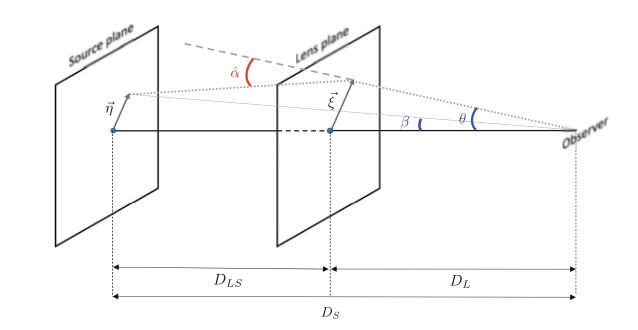
\includegraphics[width=\linewidth, keepaspectratio]{img/chapter2/lensing_sketch.png}
    \caption[Lensing system geometry]{Typical lensing system geometry.\\\small{Credits: \cite{meneghetti_introduction_2021}.}}
    \label{fig:lensing_sketch}
\end{figure}

A source located at the intrinsic angular position $\va{\b}$, which lies on the source plane at a distance $\va{\h} = \va{\b} D_S$ from the optical axis, emits photons that pass through the lens plane at a point $\va{\x} = \va{\t} D_L$. These photons are then deflected by an angle $\hat{\va{\a}}$, ultimately reaching the observer. The magnitude of this deflection is specified by \cref{eq:2.4}.
As a result of this deflection, the observer perceives the light as originating from the apparent angular position $\va{\t}$.

When the angles $\va{\t}$, $\va{\b}$, $\hat{\va{\a}}$ are small, the actual position of the source and where it appears to be located in the sky are connected by a straightforward relationship, the so-called \emph{lens equation}:
\be
\label{eq:2.9}
\va{\t} D_S = \va{\b} D_S + \hat{\va{\a}} D_{LS} \,.
\ee

Defining then the reduced deflection angle as
\be
\label{eq:2.10}
\va{\a} (\va{\t}) \equiv \dfrac{D_{LS}}{D_S} \hat{\va{\a}} (\va{\t}) \,,
\ee
\cref{eq:2.9} can be rewritten as
\be
\label{eq:2.11}
\va{\b} = \va{\t} - \va{\a} (\va{\t}) \,,
\ee
which allows to determine the intrinsic source position if the image position and the deflection angle are known. In contrast, by solving the lens equation for the unknown $\va{\t}$, it is possible to compute the image position(s) of a source placed at $\va{\b}$, lensed by a lens with a deflection field $\va{\a} (\va{\t})$.

A common choice is to write the lens equation in its dimensionless form by defining a length scale $\x_0$ on the lens plane and a corresponding length scale $\h_0 = \x_0 D_S / D_L$ on the source plane and using them to define the dimensionless (scaled) vectors
\be
\label{eq:2.12}
\vec{x} \equiv \frac{\va{\x}}{\x_0} \;,\quad \vec{y} \equiv \frac{\va{\h}}{\h_0} \,,
\ee
as well as the dimensionless deflection angle
\be
\label{eq:2.13}
\va{\a} \bp{\vec{x}} = \frac{D_L D_{LS}}{\x_0 D_S} \hat{\va{\a}} \bp{\x_0 \vec{x}} \,.
\ee

By substituting these dimensionless quantities into \cref{eq:2.11}, the dimensionless lens equation can be obtained
\be
\label{eq:2.14}
\vec{y} = \vec{x} - \va{\a} (\vec{x}) \,.
\ee


%%%%%%%%%%%%%%%%%%%%%%%%%%%%%%%%%%%%%%%%%%%%%%%%%%%%%%%
%%%%% Lensing potential and convergence %%%%%
%%%%%%%%%%%%%%%%%%%%%%%%%%%%%%%%%%%%%%%%%%%%%%%%%%%%%%%
\subsection{Lensing potential and convergence}
\label{subsec:lensing_potential_convergence}
The deflection properties of an extended distribution of matter are defined by its \emph{effective lensing potential}, namely the properly re-scaled projection on the lens plane of the three-dimensional Newtonian potential $\F$:
\be
\label{eq:2.15}
\hat{\P} (\va{\t}) = \frac{2}{c^2} \frac{D_{LS}}{D_L D_S} \int \F (D_L \va{\t}, z) \dd{z} \,.
\ee

It can be shown that the effective lensing potential satisfies two important properties:
\begin{enumerate}
    \item the gradient of $\hat{\P}$ is the reduced deflection angle:
    \be
    \label{eq:2.16}
    \va{\nabla}_\t \hat{\P} (\va{\t}) = \va{\a} (\va{\t}) \,;
    \ee

    \item the Laplacian of $\hat{\P}$ is twice the \emph{convergence} $\k$:
    \be
    \label{eq:2.17}
    \laplacian_\t \hat{\P} (\va{\t}) = 2 \k (\va{\t}) \,.
    \ee
\end{enumerate}

The convergence is defined as a dimensionless surface density
\be
\label{eq:2.18}
\k (\va{\t}) \equiv \frac{\S (\va{\t})}{\S_{cr}} \quad \mathrm{with} \quad \S_{cr} = \frac{c^2}{4 \pi G} \frac{D_S}{D_L D_{LS}} \;,
\ee
where $\S_{cr}$ is the so-called \emph{critical surface density}, a pivotal characteristic of the lens system, a function of the angular diameter distances of the lens and source, which allows to discriminate between \emph{strong} and \emph{weak} gravitational lensing regimes.

In particular, strong lensing is usually observed in regions of high mass concentration, such as the cores of galaxy clusters or around massive galaxies, when the surface mass density of the lens is comparable to or exceeds the critical surface density ($\S \geq \S_{cr}$) and the gravitational field of the lens is strong enough to produce multiple images of the source, form Einstein rings, or create arc-like structures.
On the contrary, weak lensing occurs when the surface mass density of the lens is below the critical surface density ($\S < \S_{cr}$). The gravitational effect is subtler, leading to slight distortions in the shapes of background galaxies, which can only be detected statistically over large populations of galaxies. Weak lensing does not produce multiple images or highly visible arcs but instead slightly stretches the images of background galaxies, causing shear and magnification effects.

From the previous definitions in \cref{eq:2.15,eq:2.18}, lensing quantities such as lensing potential (and therefore deflection angle) and critical surface density strongly depend on distances between observer, lens and source, which in turn depend on the source and lens redshifts.
The distance ratio
\be
\frac{D_L D_{LS}}{D_S}
\ee
is called \emph{lensing distance} and \cref{fig:lensing_distance} shows how it varies with the redshifts of source and lens.
As can be seen, the lensing distance increases with the source redshift and peaks when the lens is at an intermediate distance between the source and the observer. Clearly, the larger the lensing distance (and so the convergence), the stronger the effects generated by the lensing event.

\begin{figure}
  \centering
  \subfloat[]{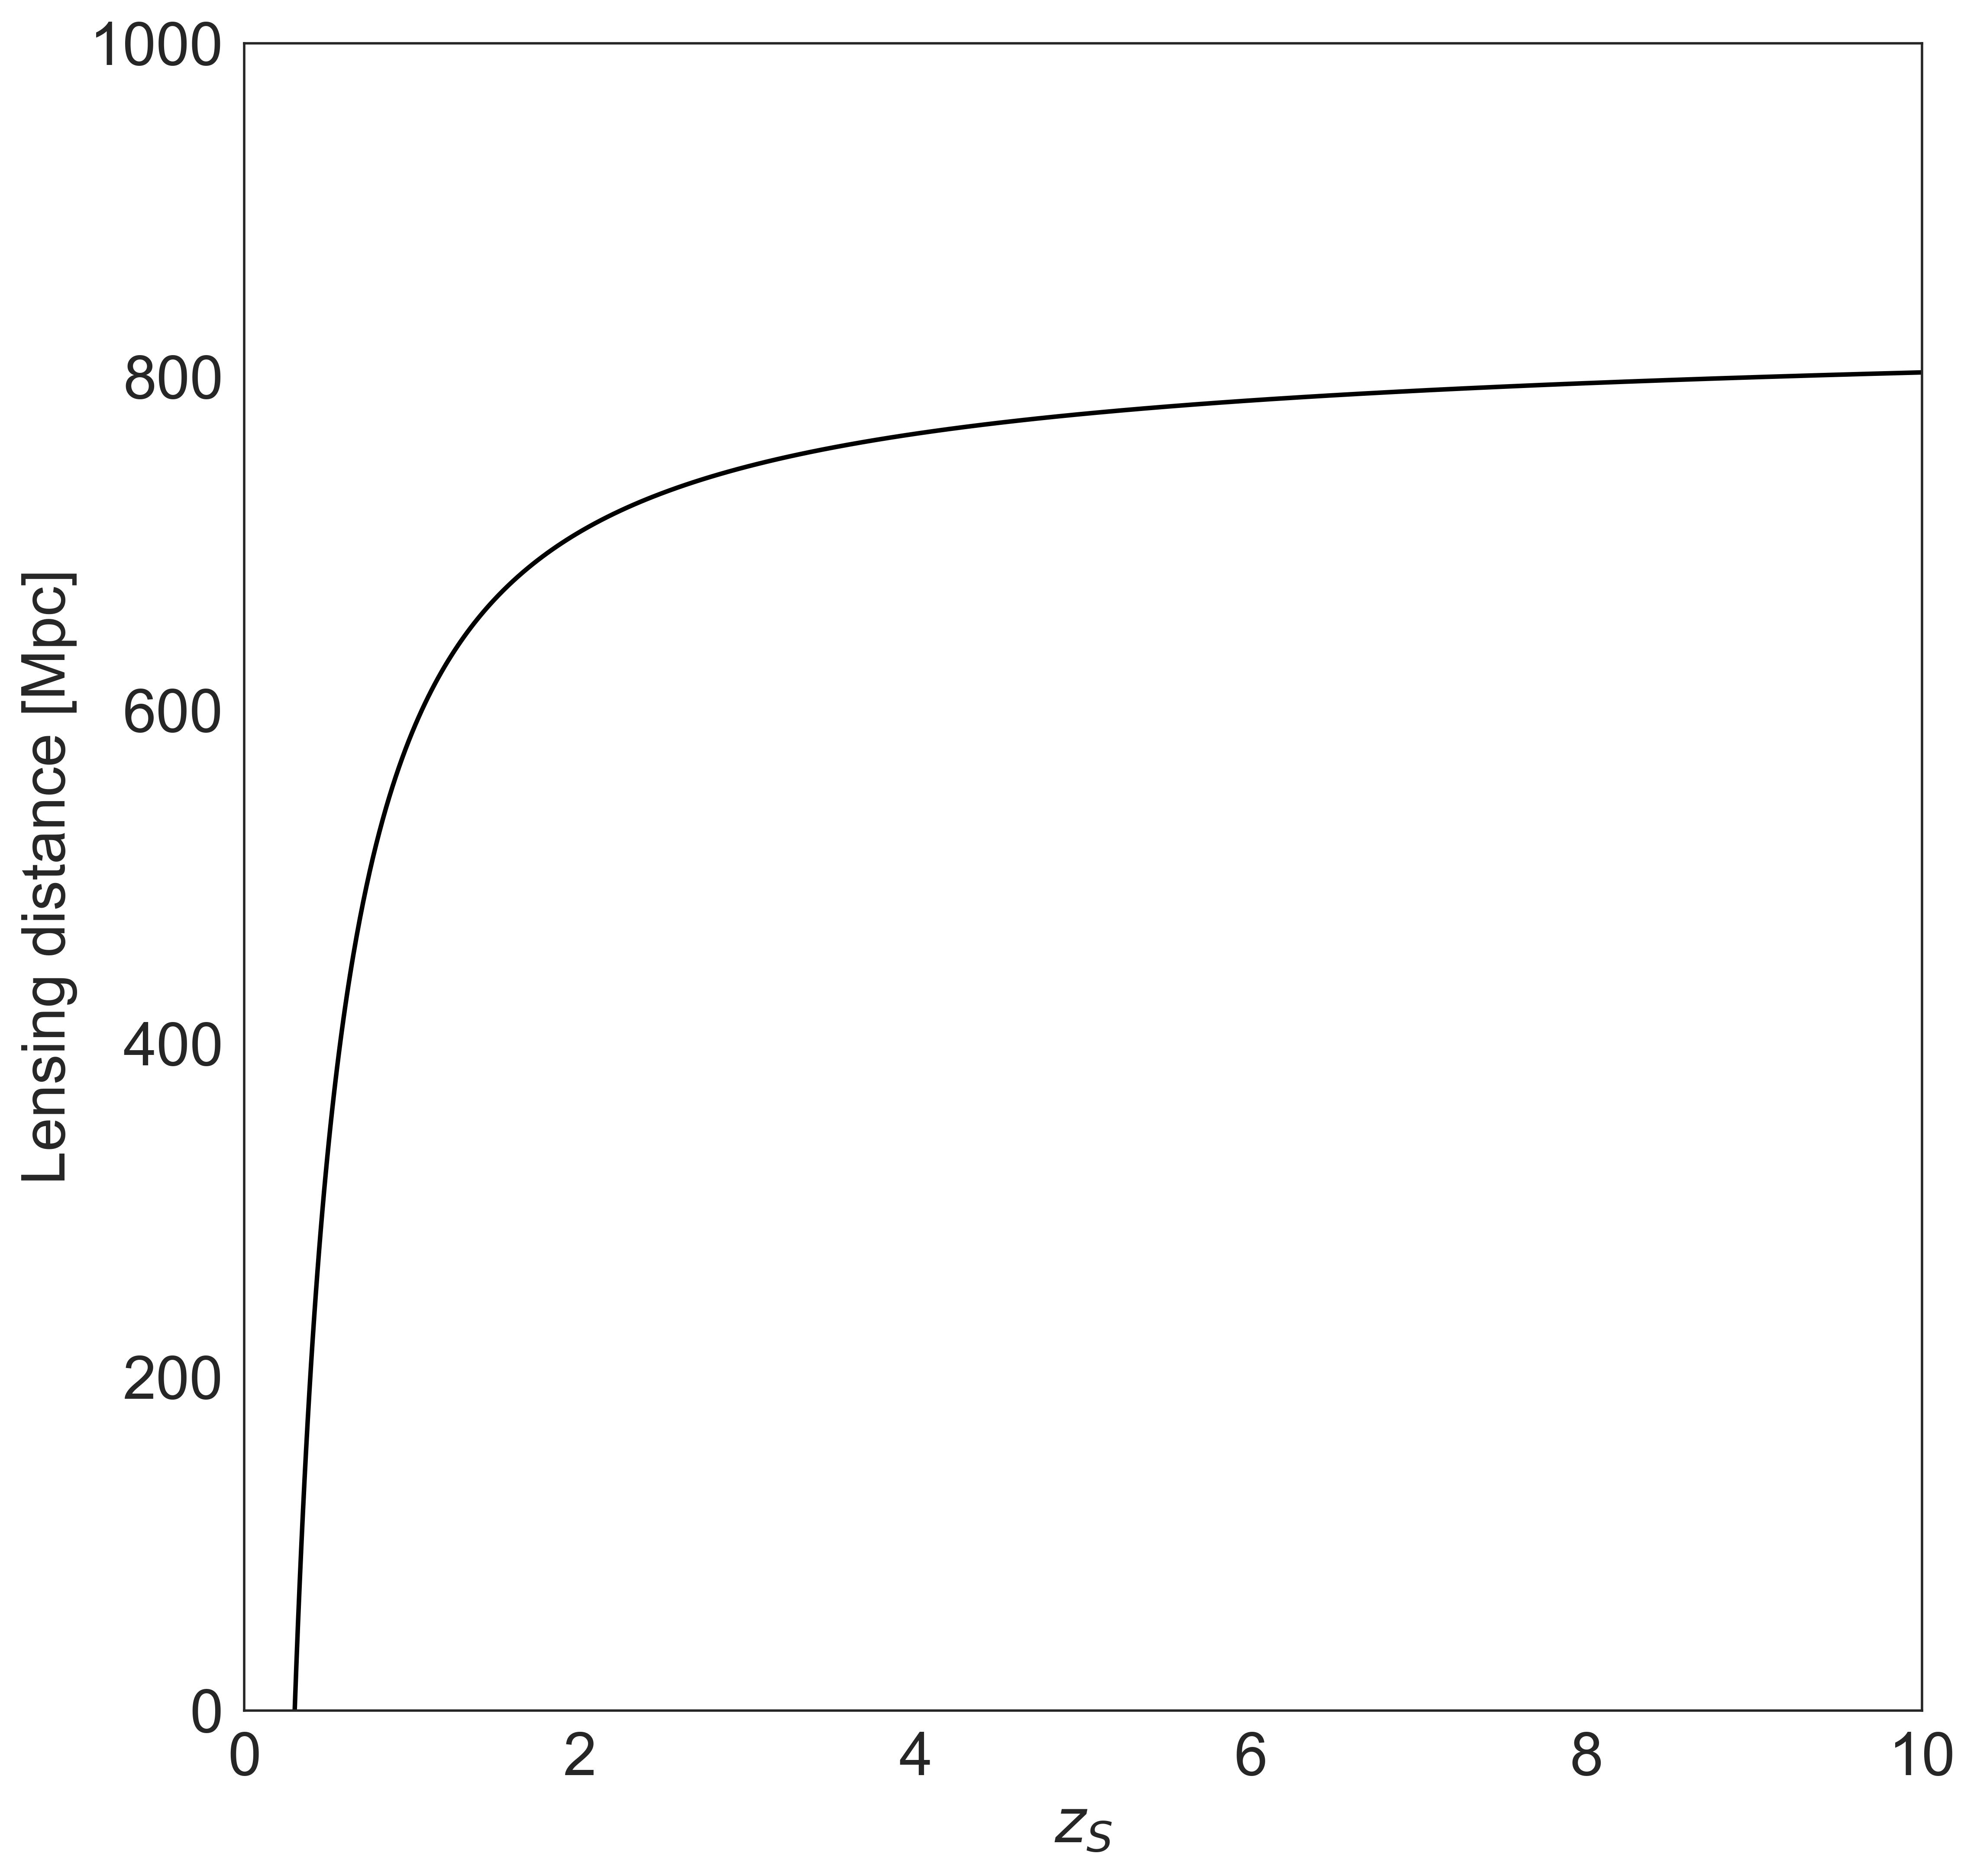
\includegraphics[width=0.5\linewidth, keepaspectratio]{img/chapter2/lensing_distance_a.png}\label{fig:lensing_distance_a}}
  \hfill
  \subfloat[]{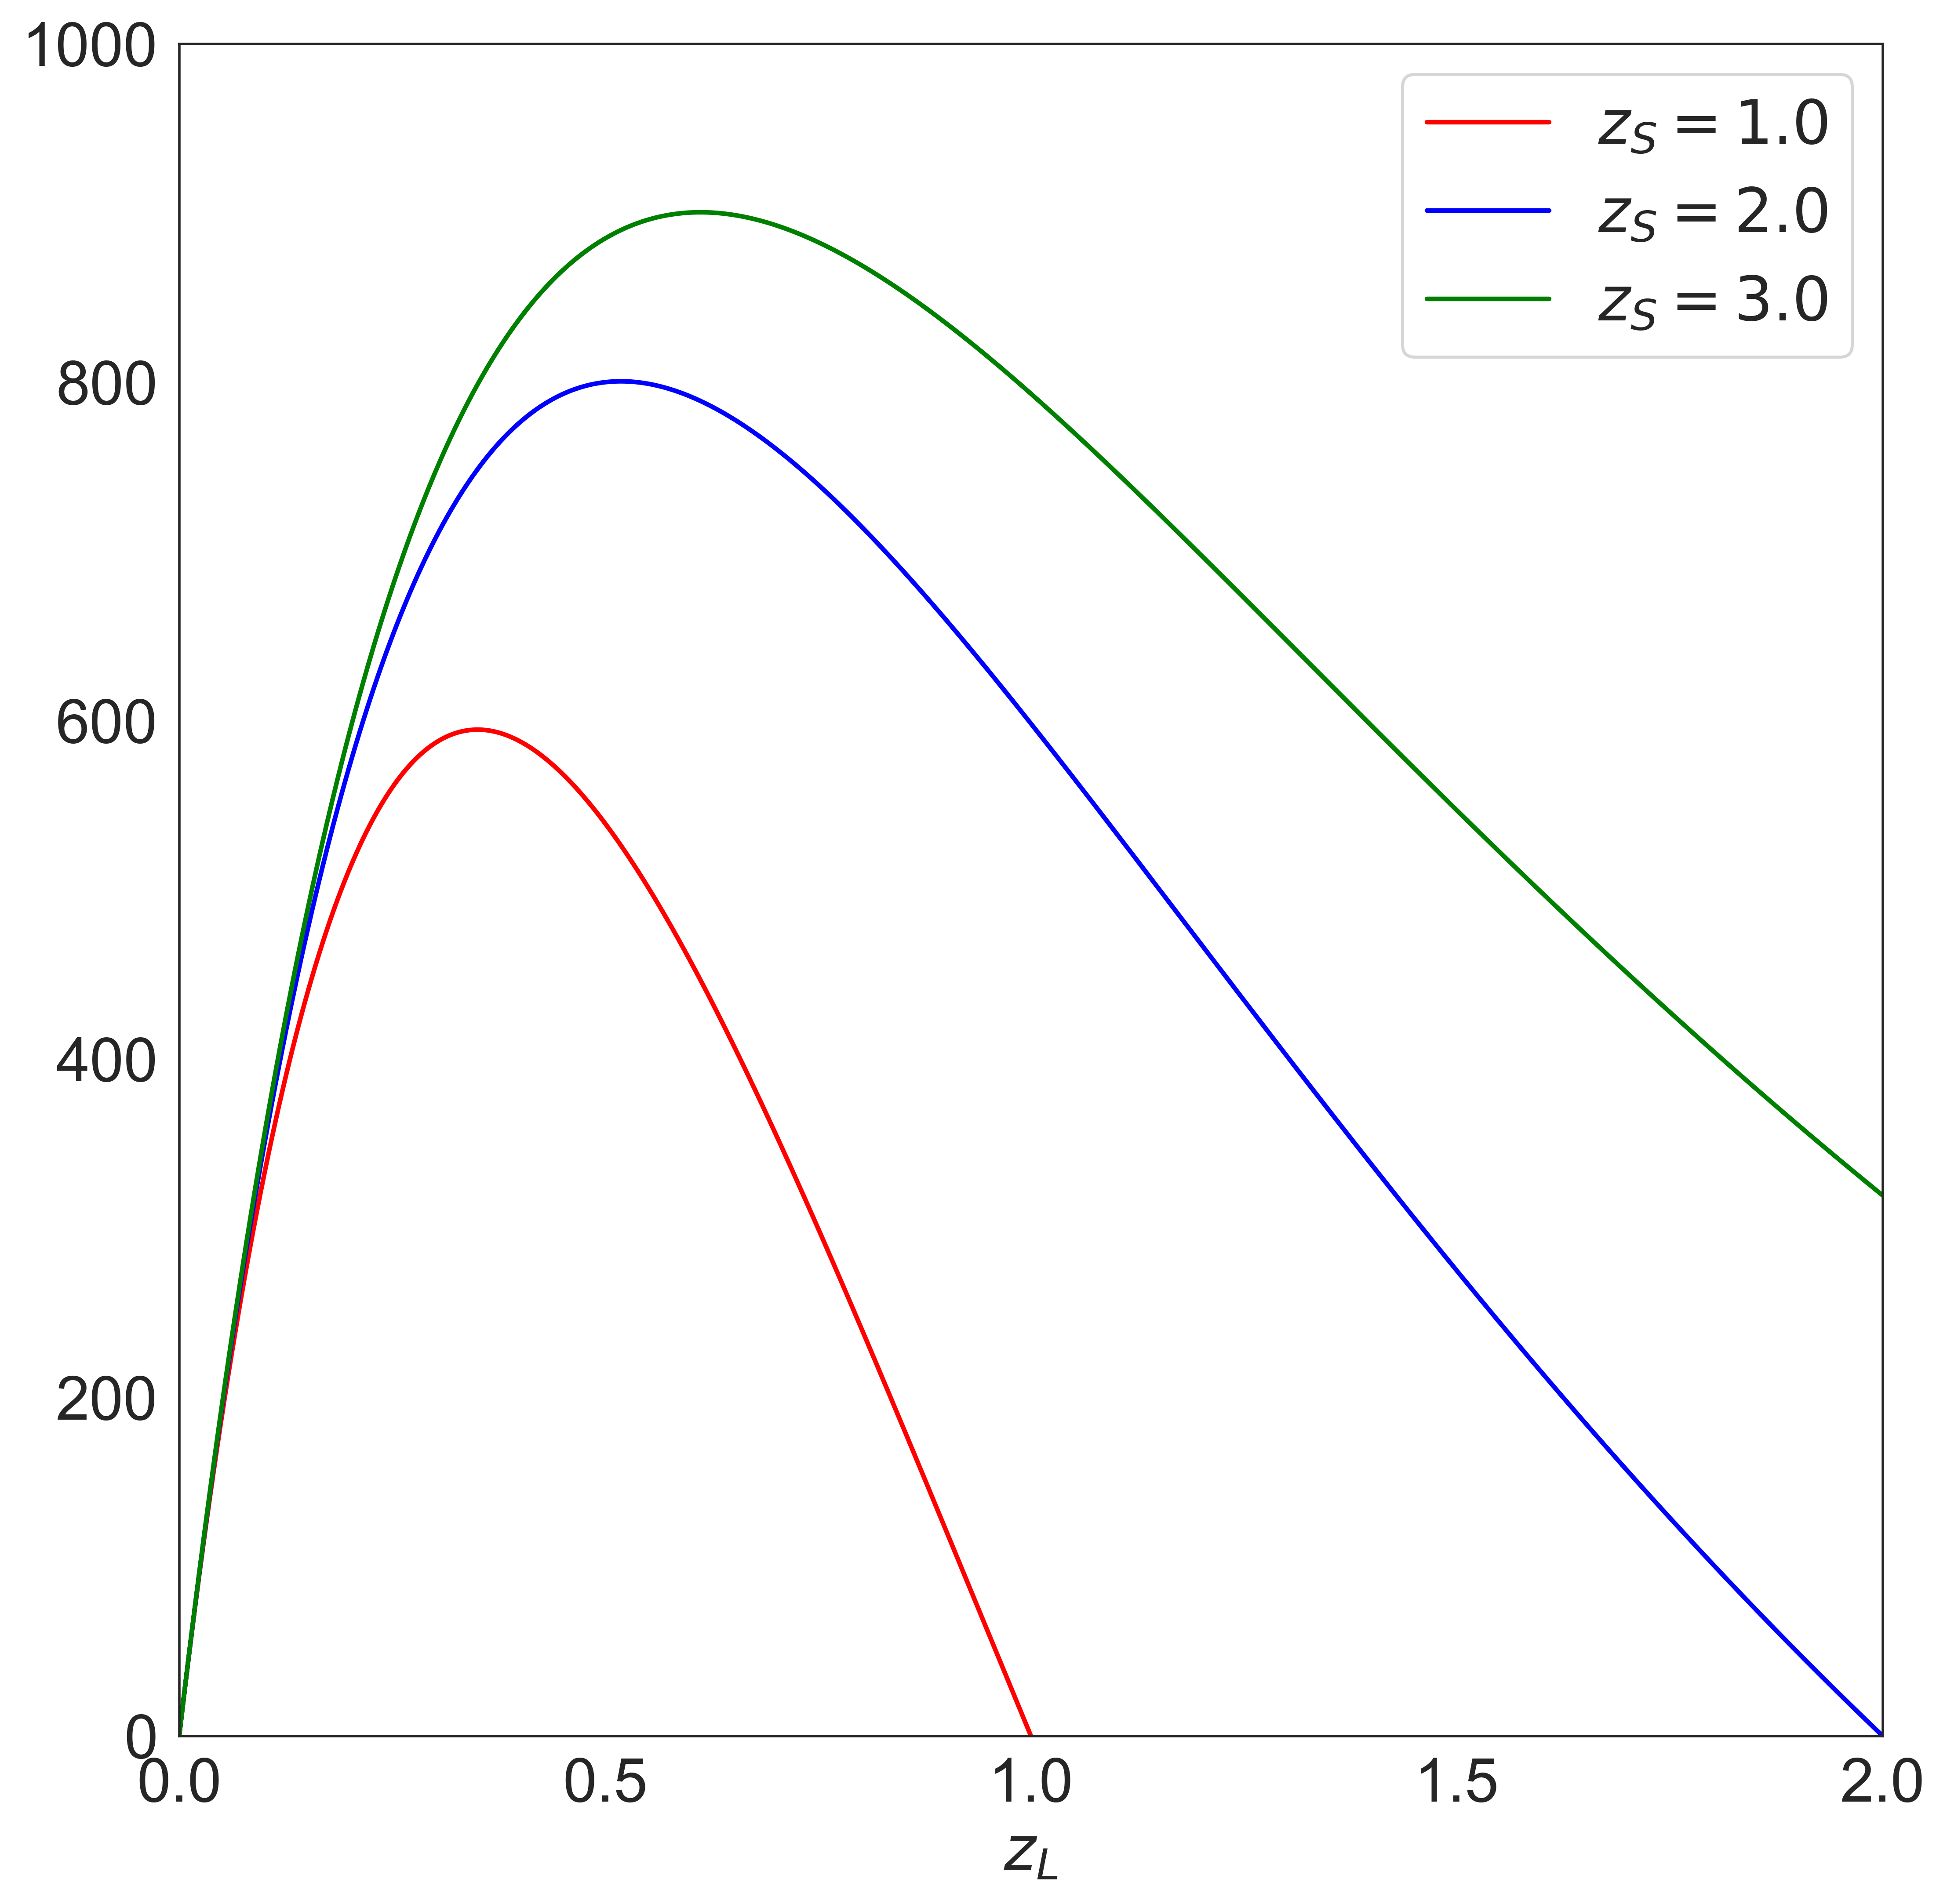
\includegraphics[width=0.5\linewidth, keepaspectratio]{img/chapter2/lensing_distance_b.png}\label{fig:lensing_distance_b}}
  \caption[Lensing distance variation with redshifts]{\protect\subref{fig:lensing_distance_a} Lensing distance variation as a function of the source redshift and \protect\subref{fig:lensing_distance_b} as a function of the lens redshift.}
  \label{fig:lensing_distance}
\end{figure}


%%%%%%%%%%%%%%%%%%%%%%%%%%%%%%%%%%%%%%%%%%%%%%%%%%%%%%%
%%%%% First-order lens mapping %%%%%
%%%%%%%%%%%%%%%%%%%%%%%%%%%%%%%%%%%%%%%%%%%%%%%%%%%%%%%
\subsection{First-order lens mapping}
\label{subsec:first_order_mapping}
A significant effect of gravitational lensing is image distortion. This alteration becomes markedly noticeable with sources of extended size. For instance, galaxies in the background can be observed as elongated arcs when they are lensed by clusters of galaxies or individual galaxies. The cause of this distortion is the varying deflection of light rays. Ideally, by solving the lens equation for every point of the extended source, the configuration of the images can be determined. Specifically, when the size of the source is significantly less than the angular scale over which the lens deflection angle field varies, the correspondence between the position of the source and the images can be approximated as linear on a local scale, allowing for a first-order approximation.

By computing the distance between two points $\va{\b}$ and $\va{\b}^\prime = \va{\b} + \dd{\va{\b}}$ on the source plane, it is possible to define a linear mapping between the source and the lens plane, described by the Jacobian matrix
\be
\label{eq:2.19}
A \equiv \frac{\partial \va{\b}}{\partial \va{\t}} = \bp{\d_{ij} - \frac{\partial \a_i (\va{\t})}{\partial \t_i}} = \bp{\d_{ij} - \frac{\partial^2 \hat{\P} (\va{\t})}{\partial \t_i \partial \t_j}} \,.
\ee

This metric is a second-rank symmetric tensor called the \emph{lensing Jacobian} and can be divided into an isotropic and an anisotropic part:
\begin{subequations}
\begin{align}
    \label{eq:2.20a}
    A_{iso, ij} & = \frac{1}{2} \Tr A \d_{ij} = \bp{1 - \frac{1}{2} \laplacian \hat{\P}} \d_{ij} = \bp{1 - \k} \d_{ij} \,,
    \\
    \label{eq:2.20b}
    A_{aniso, ij} & = A_{ij} - \frac{1}{2} \Tr A \d_{ij} = \begin{pmatrix} -\frac{1}{2} \bp{\hat{\P}_{11} - \hat{\P}_{22}} & - \hat{\P}_{12} \\ - \hat{\P}_{12} & \frac{1}{2} \bp{\hat{\P}_{11} - \hat{\P}_{22}} \end{pmatrix} \,.
\end{align}
\end{subequations}

It is possible to describe the anisotropic component of the lensing Jacobian by defining the \emph{shear} tensor $\G$, a 2x2 symmetric, traceless tensor, usually written in the form of a pseudo-vector $\va{\g} = (\g_1, \g_2)$, whose components are:
\begin{subequations}
\begin{align}
    \label{eq:2.21a}
    \g_1 & = \frac{1}{2} \bp{\hat{\P}_{11} - \hat{\P}_{22}}  \,,
    \\
    \label{eq:2.21b}
    \g_2 & = \hat{\P}_{12} = \hat{\P}_{21} \,.
\end{align}
\end{subequations}

The shear tensor has eigenvalues $\pm \sqrt{\g_1^2 + \g_2^2} = \pm \g$ and, representing the direction of the eigenvector corresponding to the positive eigenvalue with $\f$, $\G$ can be written as:
\be
\label{eq:2.22}
\G = \begin{pmatrix} \g_1 & \g_2 \\ \g_2 & - \g_1 \end{pmatrix} = \g \begin{pmatrix} \cos{2\f} & \sin{2\f} \\ \sin{2\f} & - \cos{2\f} \end{pmatrix} \,.
\ee

Summarizing, from \cref{eq:2.20a,eq:2.20b} and considering this last definition of $\G$, the lensing Jacobian becomes
\be
\label{eq:2.23}
A = (1 - \k) 
    \begin{pmatrix} 1 & 0 \\ 0 & 1 \end{pmatrix} - \g \begin{pmatrix} \cos{2\f} & \sin{2\f} \\ \sin{2\f} & - \cos{2\f} \end{pmatrix} = \begin{pmatrix} 1 - \k - \g_1  & - \g_2 \\ - \g_2 & 1 - \k + \g_1 \end{pmatrix} \,.
\ee

From the last expression of the lensing Jacobian, it can be seen that the first-order mapping is characterized by two parts. The first term, depending on the convergence, describes an isotropic transformation of the source image, which is therefore expanded or contracted by the same factor in all directions.
Instead, the second term describes an anisotropic transformation dependent on the shear, and thus causes distortions of the source image along a specific direction, given by the angle $\f$. More precisely, the image size is increased compared to the source in the direction of the eigenvectors of $A$ with eigenvalue $\g$, and decreased in the perpendicular direction. The amounts of these magnifications and de-magnifications are given by the inverse of the tangential and radial eigenvalues, namely $\l_t = 1 - \k - \g$ and $\l_r = 1 - \k + \g$.

\begin{figure}
    \centering
    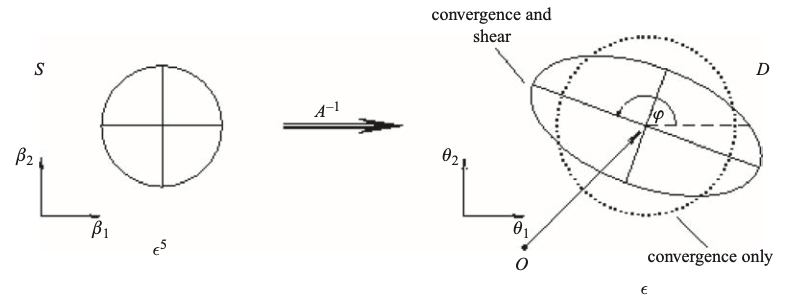
\includegraphics[width=\linewidth, keepaspectratio]{img//chapter2/convergence_shear.png}
    \caption[Convergence and shear distortion on circular source]{Distortion effects due to convergence and shear on a circular source.\\\small{Credits: \cite{mediavilla_lensing_2016}.}}
    \label{fig:convergence_shear}
\end{figure}

As an example, \cref{fig:convergence_shear} shows how a circular source of radius $r$ would be distorted by convergence and shear effects. Due to the convergence term, the source is mapped to a larger (or smaller) circle, whose radius is $r / (1 - \k)$.\\Due to the shear term, the circle is further elongated in the direction given by the angle $\f$ and contracted in the perpendicular direction to form an ellipse. 

\begin{figure}
    \centering
    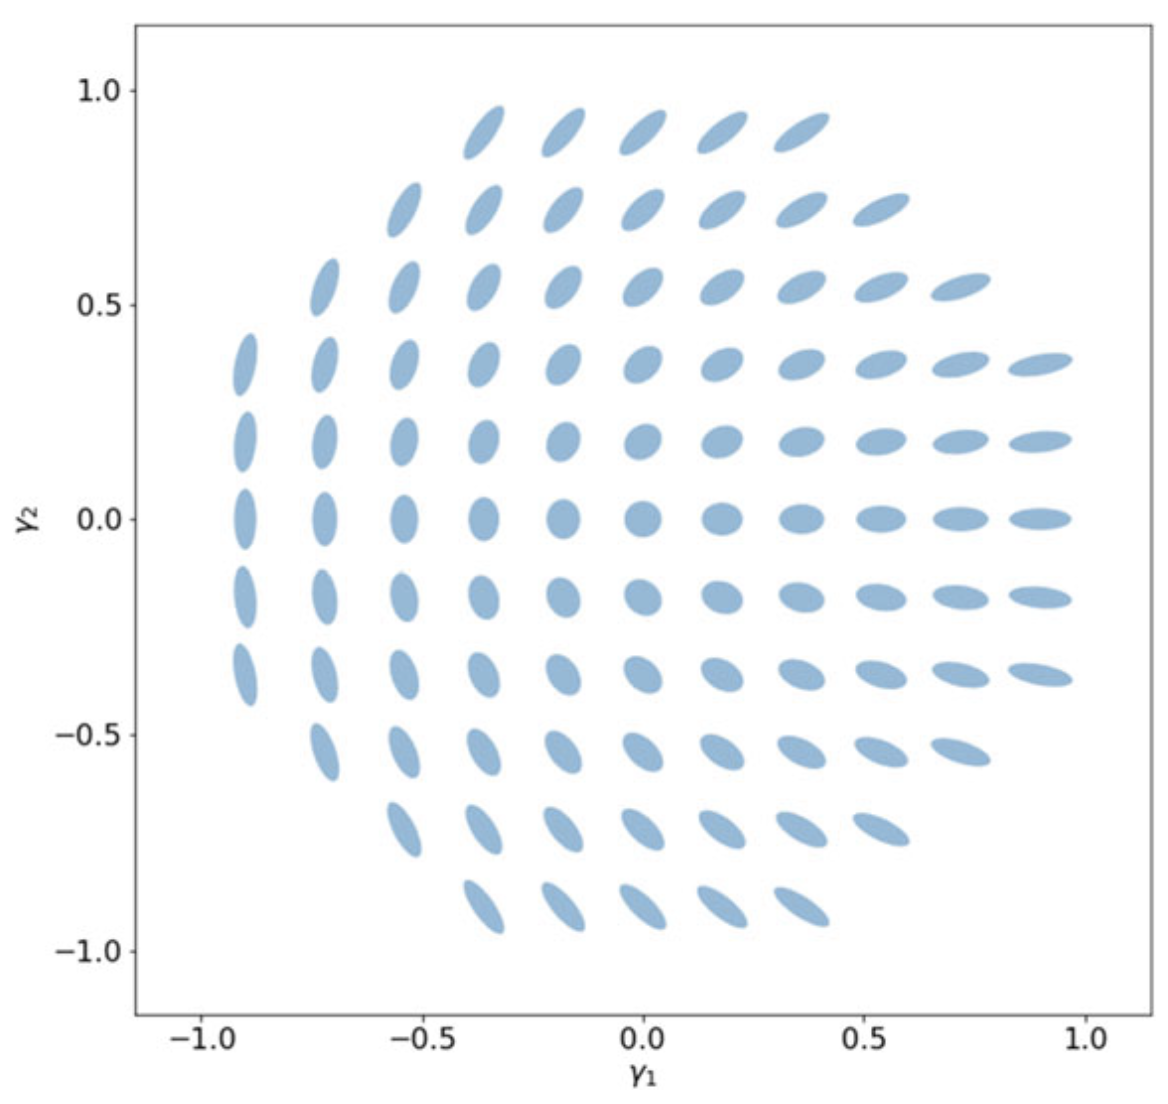
\includegraphics[width=0.7\linewidth]{img//chapter2/shear_orientations.png}
    \caption[Images orientations according to different combinations of $\g_1$ and $\g_2$]{Images orientations according to different combinations of $\g_1$ and $\g_2$.\\\small{Credits: \cite{meneghetti_introduction_2021}}.}
    \label{fig:shear_orient}
\end{figure}

This effect can be understood considering the circular source isophotes, described by
\be
\label{eq:source_isoph}
\b_1^2 + \b_2^2 = r^2 \,.
\ee

It is always possible to choose a reference frame where the Jacobian matrix is diagonal, so that the lens equation for a circular source is
\begin{subequations}
\begin{align}
    \label{eq:circu_lens1}
    \b_1 = (1 - \k - \g) \t_1 \,,
    \\
    \label{eq:circu_lens2}
    \b_2 = (1 - \k + \g) \t_2 \,.
\end{align}
\end{subequations}

By substituting these values into \cref{eq:source_isoph} the equation of the isophotes becomes
\be
\label{eq:ellipse_isoph}
(1 - \k - \g)^2 \t_1^2 + \b_2 = (1 - \k + \g)^2 \t_2^2 = r^2 \,,
\ee
which represents the equation for an ellipse, with major and minor axes $a = r/\l_t$ and $b = r/\l_r$, respectively.

Moreover, the fact that the shear tensor has spin 2 translates in different distortions according to its components:
\begin{itemize}
    \item $\g_1>0$, $\g_2 = 0$: major axis of the ellipse is along $\t_1$;
    \item $\g_1=0$, $\g_2 > 0$: major axis of the ellipse forms an angle of $\pi/4$ with $\t_1$;
    \item $\g_1<0$, $\g_2 = 0$: major axis of the ellipse is perpendicular to $\t_1$;
    \item $\g_1=0$, $\g_2 < 0$: major axis of the ellipse forms and angle of $3\pi/4$ with $\t_1$.
\end{itemize}

\Cref{fig:shear_orient} shows how images orientations are affected by these combinations of $\g_1$ and $\g_2$ and many more.


%%%%%%%%%%%%%%%%%%%%%%%%%%%%%%%%%%%%%%%%%%%%%%%%%%%%%%%
%%%%% Magnification %%%%%
%%%%%%%%%%%%%%%%%%%%%%%%%%%%%%%%%%%%%%%%%%%%%%%%%%%%%%%
\subsection{Magnification}
\label{subsec:magnification}
One of the most important features introduced by gravitational lensing is the \emph{magnification} effect: through the lens equation, the solid angle $\d \b^2$ is mapped to the solid angle $\d \t^2$. In the absence of photon emission or absorption, the Liouville theorem states that the surface brightness of a source remains constant as it passes through the lensing field. Thus, the change in the solid angle under which the source is observed implies that the flux received is magnified (or demagnified).
From \cref{eq:2.19}, the magnification introduced by the lensing is given by the inverse of the determinant of the Jacobian matrix. For this reason, the matrix $M = A^{-1}$ is called the \emph{magnification tensor} and therefore:
\be
\label{eq:2.24}
\m \equiv \det M = \frac{1}{\det A} = \frac{1}{(1- \k)^2 - \g^2} \,,
\ee
while the relation between intrinsic and observed flux can be written
\be
\label{eq:2.25}
F_\n = \int_I I_\n (\va{\t}) \dd^2{\t} = \int_S I_\n^S (\va{\b}(\va{\t})) \m (\va{\t}) \dd^2{\b} \,,
\ee
where the first integral is over the image plane and the second over the source plane.
From \cref{eq:2.24}, it is possible to define $\m_t = \l_t^{-1}$ and $\m_r = \l_r^{-1}$, the so-called \emph{tangential} and \emph{radial} magnification factors, so that $\m = \m_t \m_r$.

Since both convergence and shear (and therefore magnification) are functions of the position on the lens plane $\va{\t}$, there exists a set of critical points where $\det A = 0$, which means either $\l_t = 0$ or $\l_r = 0$. The ensemble of these points defines the \emph{critical lines}, along which the magnification diverges. By mapping the critical lines to the source plane through the lens equation, new sets of points are obtained, which are called \emph{caustics}.
The shape of these critical lines and caustics varies with the mass distribution of the lens. Some examples for different mass distributions are shown in \cref{fig:caustics_critlines}.

\begin{figure}
    \centering
    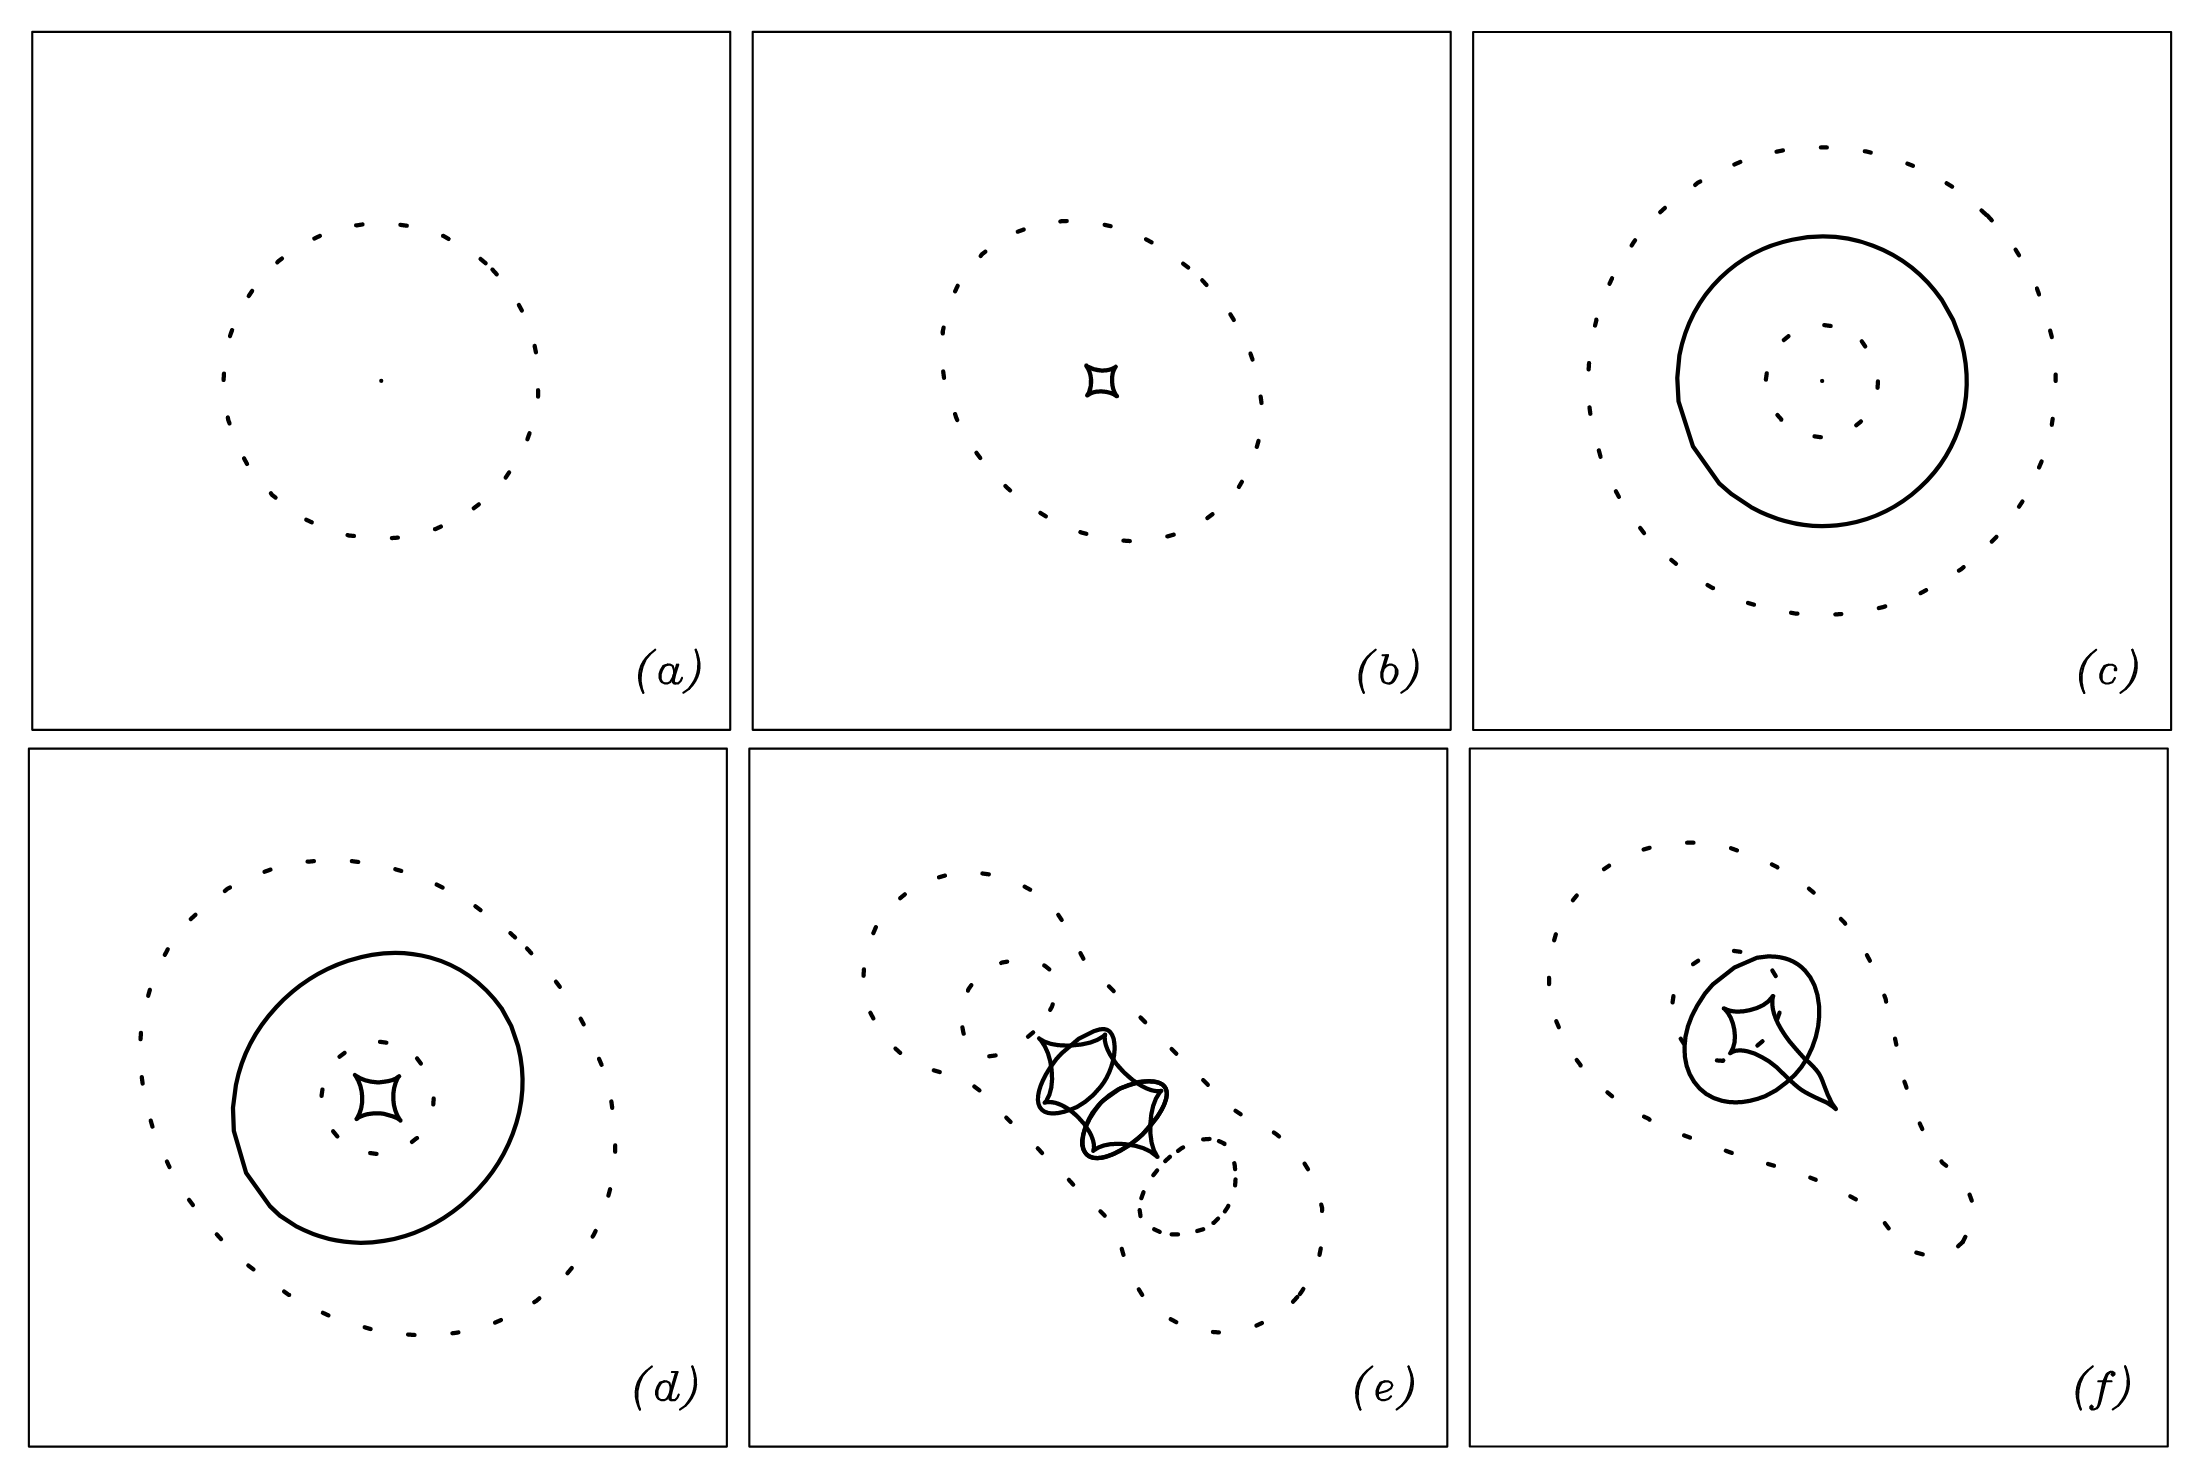
\includegraphics[width=0.6\linewidth, keepaspectratio]{img//chapter2/caustics_critlines.png}
    \caption[Caustics and critical lines shapes]{Caustics (solid) and critical lines (dashed) for different mass models: (a) a singular isothermal circular mass distribution generates only the critical lines, in particular the radial critical line is the central point and the tangential critical line is the circle; (b) a singular isothermal elliptical lens produces a tangential caustic (astroid) and the corresponding elliptical tangential critical line; (c) a circular and (d) elliptical mass distribution with shallower inner slope than the isothermal mass distribution generates both the critical lines and caustics; a bimodal mass distribution with two clumps of equal (e) or unequal (d) mass produces more complex critical lines and caustics.\\\small{Credits: \cite{kneib_cluster_2011}.}}
    \label{fig:caustics_critlines}
\end{figure}


%%%%%%%%%%%%%%%%%%%%%%%%%%%%%%%%%%%%%%%%%%%%%%%%%%%%%%%
%%%%% Time-delay and multiple images %%%%%
%%%%%%%%%%%%%%%%%%%%%%%%%%%%%%%%%%%%%%%%%%%%%%%%%%%%%%%
\subsection{Time-delay and multiple images}
\label{subsec:time_delay_images}
The deflection of light by a gravitational potential causes a delay in the travel time of light between the source and the observer, resulting in the appearance of multiple images of the source on the lens plane at different times.
This time delay has two components: one is geometrical, due to the different path length of the deflected light rays compared to the unperturbed ones, and one is gravitational, due to the effective speed of light in the presence of a gravitational potential.

The total time delay as a function of the position of the image, for a given source and lens, can be described by a surface known as \emph{time delay surface}:
\be
\label{eq:2.26}
t (\va{\t}) = t_{geom} + t_{grav} = \frac{(1 + z_L)}{c} \frac{D_L D_S}{D_{LS}} \left[ \frac{1}{2} (\va{\t} - \va{\b})^2 - \hat{\P} (\va{\t}) \right] = \frac{D_{\D t}}{c} \tau (\va{\t}) \,,
\ee
where $z_L$ is the lens redshift and the quantities
\begin{subequations}
\begin{align}
    \label{eq:2.27a}
    D_{\D t} & = (1 + z_L) \frac{D_L D_S}{D_{LS}} \,,
    \\
    \label{eq:2.27b}
    \tau (\va{\t}) & = \frac{1}{2} (\va{\t} - \va{\b})^2 - \hat{\P} (\va{\t})
\end{align}
\end{subequations}
are called \emph{time delay distance} and \emph{Fermat potential}, respectively.

The lens equation can be obtained taking the gradient of \cref{eq:2.26}:
\be
\label{eq:2.28}
\va{\nabla} \left[ \frac{1}{2} (\va{\t} - \va{\b})^2 - \hat{\P} (\va{\t}) \right] = 0 \,.
\ee

Therefore, the images are formed at the stationary points of the time delay surface, whose curvature is given by its Hessian matrix:
\be
\label{eq:2.29}
T_{ij} = \frac{\partial^2 t (\va{\t})}{\partial \t_i \partial \t_j} \propto (\d_{ij} - \hat{\P}_{ij}) = A_{ij} \,.
\ee

\begin{figure}[b!]
    \centering
    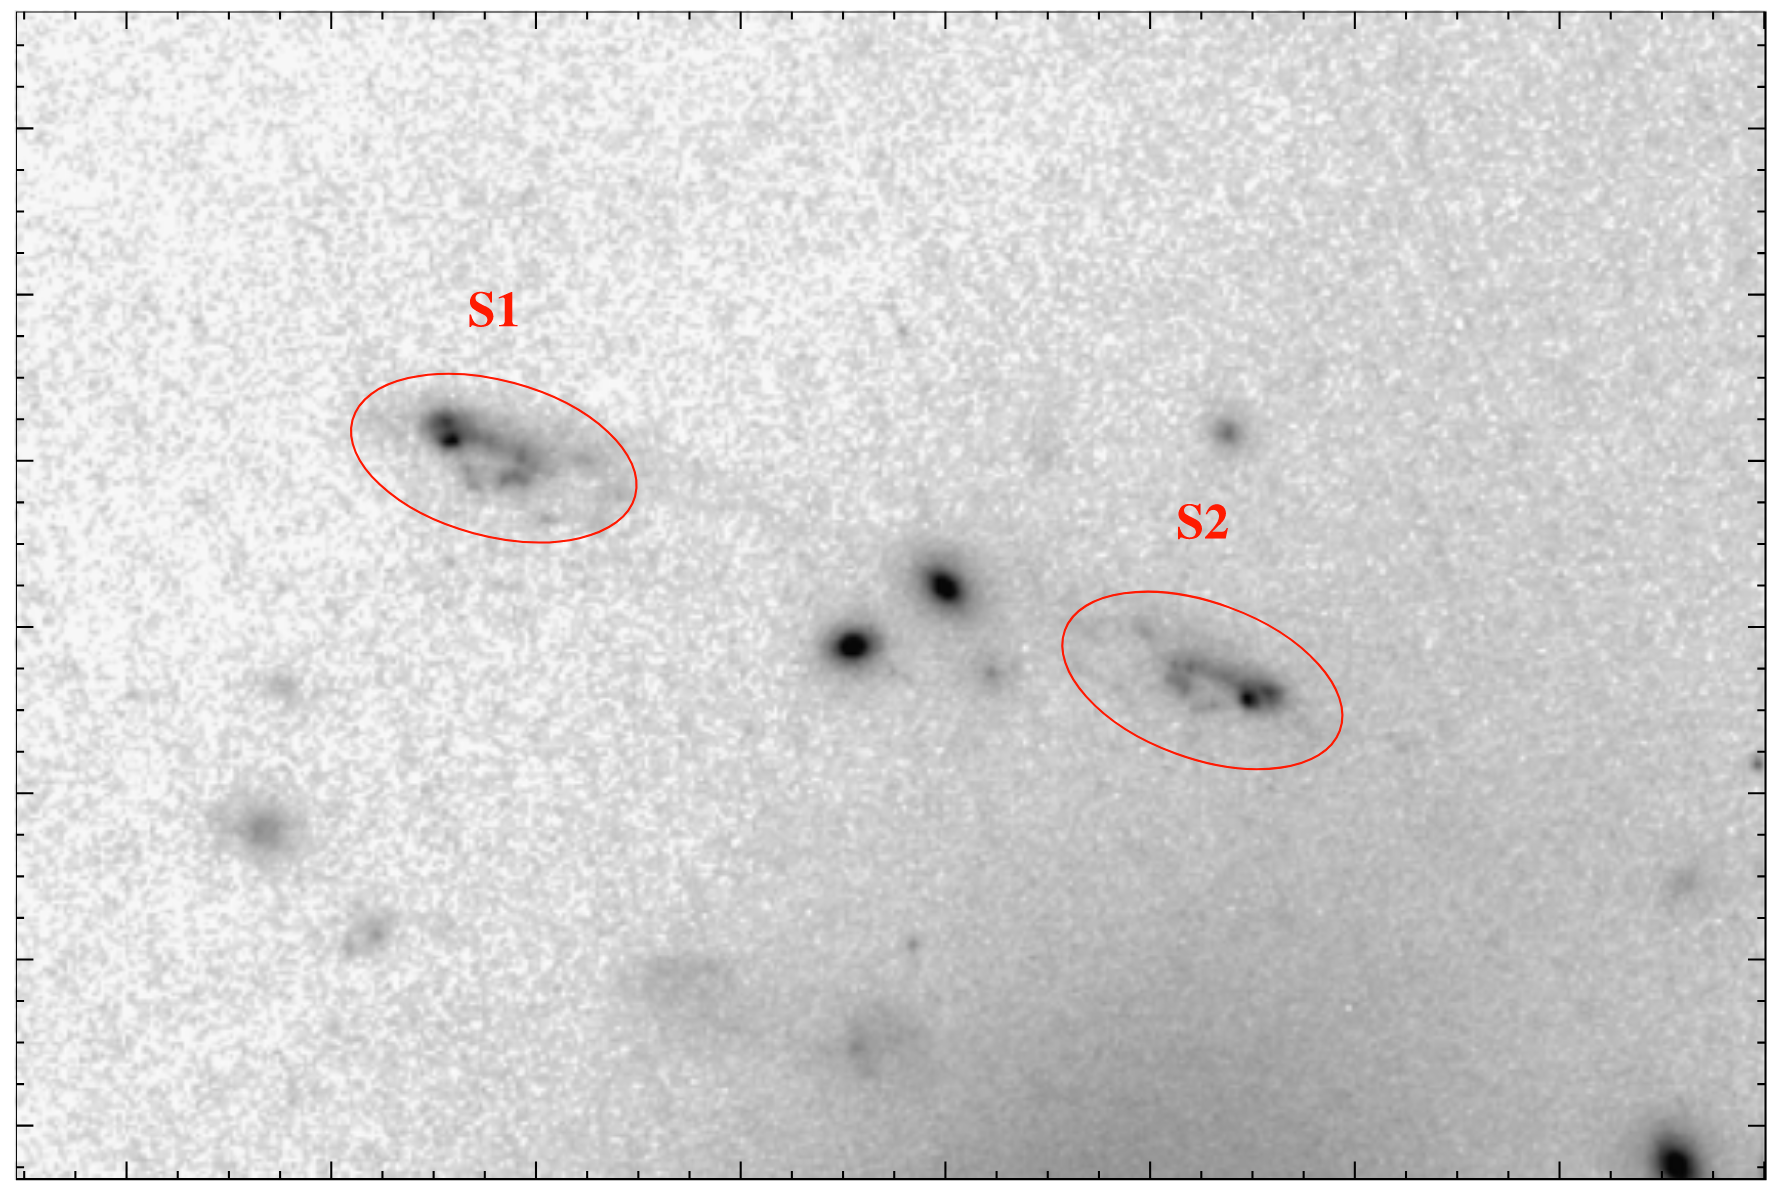
\includegraphics[width=0.9\linewidth, keepaspectratio]{img//chapter2/lensedpair.png}
    \caption[The lensed pair S1–S2 in AC114]{The lensed pair S1–S2 in AC114. This galaxy at $z = 1.867$ displays the surprising morphology of a hook, with an obvious change in parity.\\\small{Credits: \cite{kneib_cluster_2011}.}}
    \label{fig:lensedpair}
\end{figure}

The multiplicity of images in gravitational lensing is closely related to the characteristics of the time delay surface, and the configuration of this surface near stationary points offers insights into the shapes of the images and their \emph{parity}. Image parity is determined by the magnification sign: magnifications $>1$, whether positive or negative, both amplify the image. However, a positive magnification retains the original orientation of the unlensed source in the image, whereas a negative magnification results in an image with reversed parity.
Crossing a critical line results in a sign change in one of the Jacobian matrix's eigenvalues, leading to a shift in the image's parity. As a consequence, the parity of images located on opposite sides of a critical line is opposite to each other (\cref{fig:lensedpair}).
Furthermore, it can be shown that the number of images changes by two when the source crosses a caustic \citep{schneider_gravitational_1992} and that the total number of images of a generic lens is odd \citep{burke_multiple_1981}.

Different stationary points result in different types of image:
\begin{itemize}
    \item \textbf{type I images} arise at the minima of surface where both \cref{eq:2.29} eigenvalues are positive, so $\det A > 0 \,, \; \Tr A > 0$ $\rightarrow$ positive magnification;
    \item \textbf{type II images} appears at the saddle points of the surface where \cref{eq:2.29} eigenvalues have opposite signs, so $\det A < 0$ $\rightarrow$ negative magnification (\ie reversed image parity, not de-magnified);
    \item \textbf{type III images} arise at the maxima of the surface where both \cref{eq:2.29} eigenvalues are negative, so $\det A > 0 \,, \; \Tr A < 0$ $\rightarrow$ positive magnification.
\end{itemize}

\Cref{fig:timedelay1d} shows the geometrical and gravitational components of the time delay and their combination for a few positions of the source relative to the lens, considered axially symmetric. The geometric time delay is described by a parabola, and the gravitational function will vary depending on the potential considered.
In particular, for a source perfectly aligned with the center of the lens (top left of \cref{fig:timedelay3d}) there exist three stationary points, two of which (the minima) merge onto a single ring. This configuration is the so-called \emph{Einstein ring}. 

Thus, it is possible to introduce the so-called Einstein radius (\cref{fig:einsteinring}), which is properly an angle, useful to define the radius of the Einstein ring:
\be
\label{eq:2.30}
\t_E = \sqrt{\frac{4 G M(\t)}{c^2} \frac{D_{LS}}{D_L D_S}} \,.
\ee

\begin{figure}
  \centering
  \subfloat[]{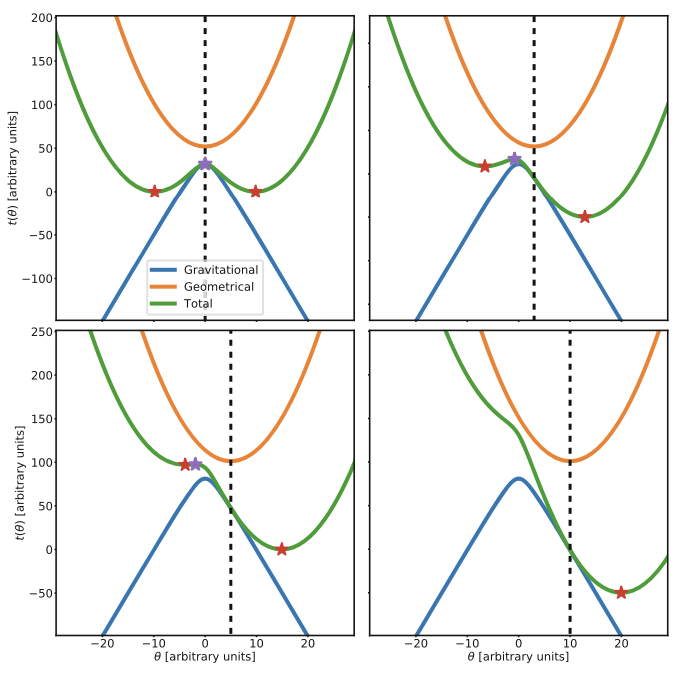
\includegraphics[width=0.5\linewidth, keepaspectratio]{img//chapter2/timedelay1d.png}\label{fig:timedelay1d}}
  \hfill
  \subfloat[]{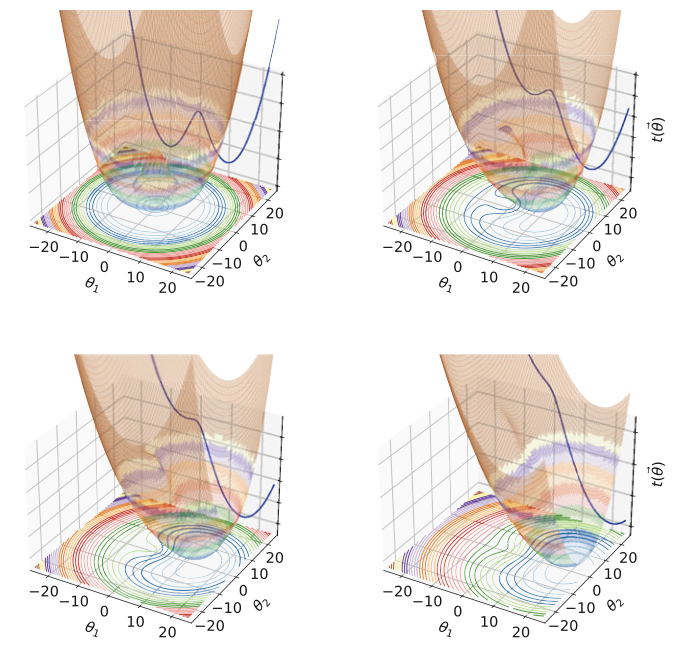
\includegraphics[width=0.5\linewidth, keepaspectratio]{img//chapter2/timedelay3d.png}\label{fig:timedelay3d}}
  \caption[Time delay functions and surfaces]{\protect\subref{fig:timedelay1d} One-dimensional time delay functions for a non-singular isothermal potential. The stars indicate the position of the images. Each panel corresponds to a different position of the source relative to the lens (dashed line). \protect\subref{fig:timedelay3d} Time delay surfaces for the same lens. Each panel corresponds to a different position of the source relative to the lens. Clearly visible Einstein ring in the top-left plot.\\\small{Credits: \cite{meneghetti_introduction_2021}.}}
  \label{fig:timedelay}
\end{figure}

\begin{figure}
    \centering
    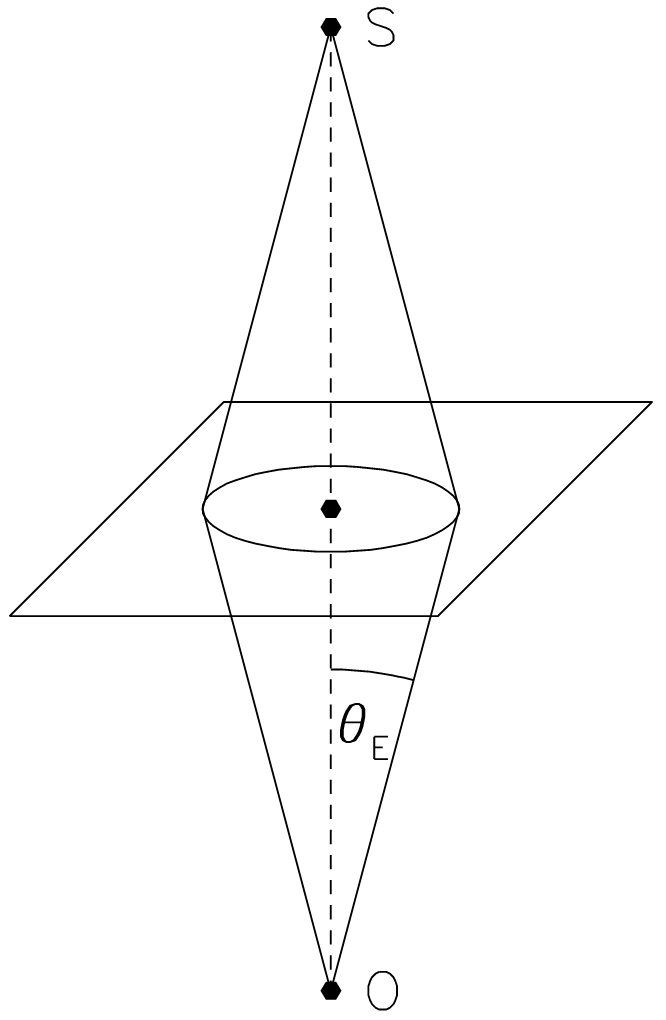
\includegraphics[width=0.22\linewidth, keepaspectratio]{img//chapter2/einsteinring.png}
    \caption[Einstein radius]{A source S exactly behind the center of an axially symmetric lens is mapped into the Einstein ring, with angular radius given by $\t_E$.\\\small{Credits: \cite{narayan_lectures_1997}.}}
    \label{fig:einsteinring}
\end{figure}